\section{Auswertung}
\label{sec:auswertung}
\subsection{Statische Methode}
\label{sec:as}

Im Folgenden werden die nach Kapitel \ref{sec:statisch} aufgenommenen Messdaten der statischen Methode ausgewertet.
In Abbildung \ref{fig:temp} sind die Messdaten der fernen Thermoelemente für die verschiedenen Stäbe als ($t$-$T$)-Diagramm dargestellt.

\begin{figure}[H]
    \centering
    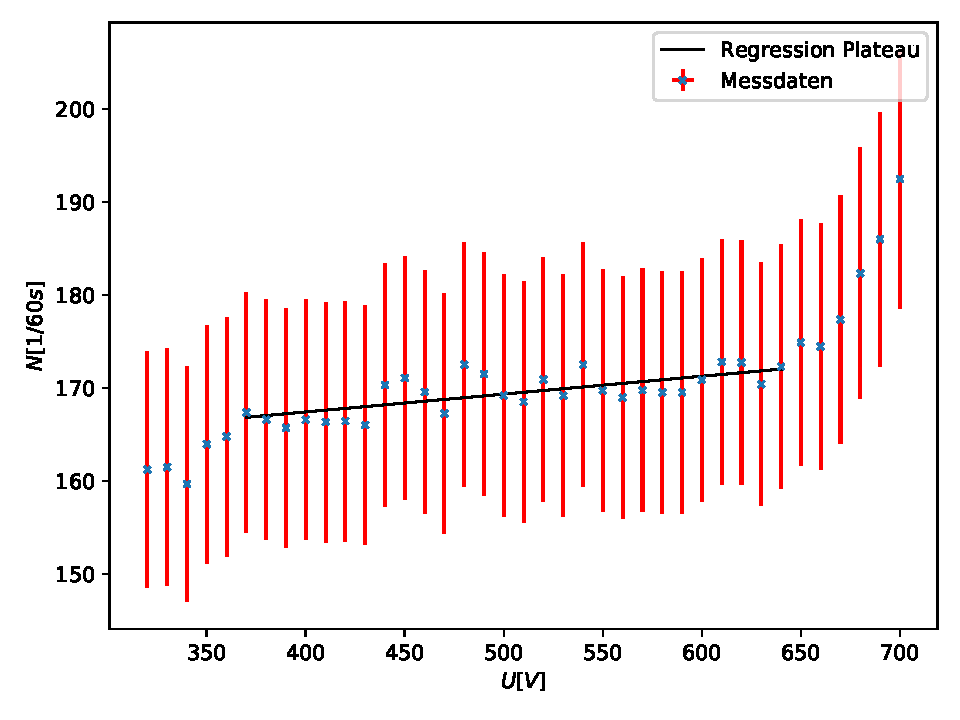
\includegraphics[width=\textwidth]{build/plot1.pdf}
    \caption{Temperaturverlauf der fernen Thermoelemente.}
    \label{fig:temp}
\end{figure}

\noindent
Es ist zu erkennen, dass alle Graphen zu Beginn exponentiell ansteigen und dann stark abflachen. Dabei nimmt die Temperatur von Aluminium
am schnellsten zu, gefolgt von dem breiteren Messingstab. Die Temperaturkurve des Edelstahls steigt dabei noch langsamer als
die des schmaleren Messingstabes. Nach dem Abflachen der Kurven ist die Steigung für alle Metalle ähnlich. In Tabelle \ref{tab:T(700)}
sind die Temperaturen der fernen Thermoelemente nach einer Messzeit von $t=\SI[]{700}[]{\second}$ aufgelistet.

\begin{table}[H]
  \centering
      \caption{Temperaturen an den fernen Thermoelementen bei $t=\SI{700}{\second}$.}
      \label{tab:T(700)}
      \sisetup{table-format=2.2}
      \begin{tabular}{S S S S}
        \toprule
        {$T_\text{Messing,b}[\si{\celsius}]$} & {$T_\text{Messing,s}[\si{\celsius}]$} & {$T_\text{Alu}[\si{\celsius}]$} & {$T_\text{Stahl} [\si{\celsius}]$}\\
        \midrule
        43.26&     36.41&     47.11&     32.68\\
        \bottomrule
      \end{tabular}
    \end{table}
\noindent
Die Messdaten aus Tabelle \ref{tab:T(700)} stützen die Beobachtung von Abbildung \ref{fig:temp}, dass Aluminium die größte und Edelstahl
die geringste Wärmeleitfähigkeit besitzt.
\\\noindent
Die Wärmeströme $\Phi=\Delta Q/\Delta t$ werden mit Gleichung \eqref{eqn:wärmemenge} berechnet. Dafür werden für fünf Zeitpunkte
$t\in\{100, 200, 300, 400, 500\}$ die Temperaturdifferenzen zwischen den fernen und nahen Thermoelementen berechnet. Die Querschnittsfläche
$A$ ist dabei das Produkt aus der Breite und der Höhe der Metallstäbe. Diese Werte werden aus der Versuchsanleitung \cite{AP01} entnommen.
Dabei ergibt sich
\begin{align*}
  A_{breit} &=\SI{48 e-6}{\square\metre}\\
  A_{schmal}&=\SI{28 e-6}{\square\metre} \; .
\end{align*}
Durch Messung ergibt sich für den Abstand $\Delta x$ zwischen den Thermoelementen $\Delta x=\SI{0.03}{\metre}$.
In Tabelle \ref{tab:wärmestrom} sind die Wärmeströme der Metalle für die verschiedenen Zeiten aufgelistet.

\begin{table}[H]
  \centering
      \caption{Wärmestrom für Messing, Aluminium und Edelstahl zu verschiedenen Zeiten.}
      \label{tab:wärmestrom}
      \sisetup{table-format=3.2}
      \begin{tabular}{S[table-format=3.0] S S[table-format=1.2] S S[table-format=1.2] S S[table-format=1.2] S S[table-format=1.2]}
        \toprule
        &
        \multicolumn{2}{c}{Messing, breit}&
        \multicolumn{2}{c}{Messing, schmal}&
        \multicolumn{2}{c}{Aluminium} &
        \multicolumn{2}{c}{Edelstahl}\\
        \cmidrule(lr){2-3}\cmidrule(lr){4-5}\cmidrule(lr){6-7}\cmidrule(lr){8-9}
        {$t [\si{\second}]$} &
        {$T_1 [\si{\kelvin}]$} & {$\Phi[\si{\watt}]$} &
        {$T_4 [\si{\kelvin}]$} & {$\Phi[\si{\watt}]$} &
        {$T_5 [\si{\kelvin}]$} & {$\Phi[\si{\watt}]$} &
        {$T_8 [\si{\kelvin}]$} & {$\Phi[\si{\watt}]$} \\
        \midrule
        100 & 300.3 & 1.09 & 296.6 & 0.40 & 305.4 & 0.79 & 293.4 & 0.32 \\
        200 & 306.6 & 0.80 & 300.7 & 0.35 & 312.1 & 0.33 & 296.7 & 0.38 \\
        300 & 310.2 & 0.65 & 303.5 & 0.32 & 315.2 & 0.16 & 299.4 & 0.36 \\
        400 & 312.5 & 0.57 & 305.5 & 0.29 & 317.0 & 0.10 & 301.4 & 0.34 \\
        500 & 314.1 & 0.53 & 307.1 & 0.28 & 318.3 & 0.07 & 303.1 & 0.33 \\
        \bottomrule
      \end{tabular}
    \end{table}

\noindent
In Abbildung \ref{fig:diff} ist die Temperaturdifferenz $\Delta T_{St}$ zwischen den nahen und den fernen Thermoelementen in Abhängigkeit
von der Zeit $t$ für den breiten Messing- und den Edelstahlstab dargestellt.

\begin{figure}[H]
    \centering
    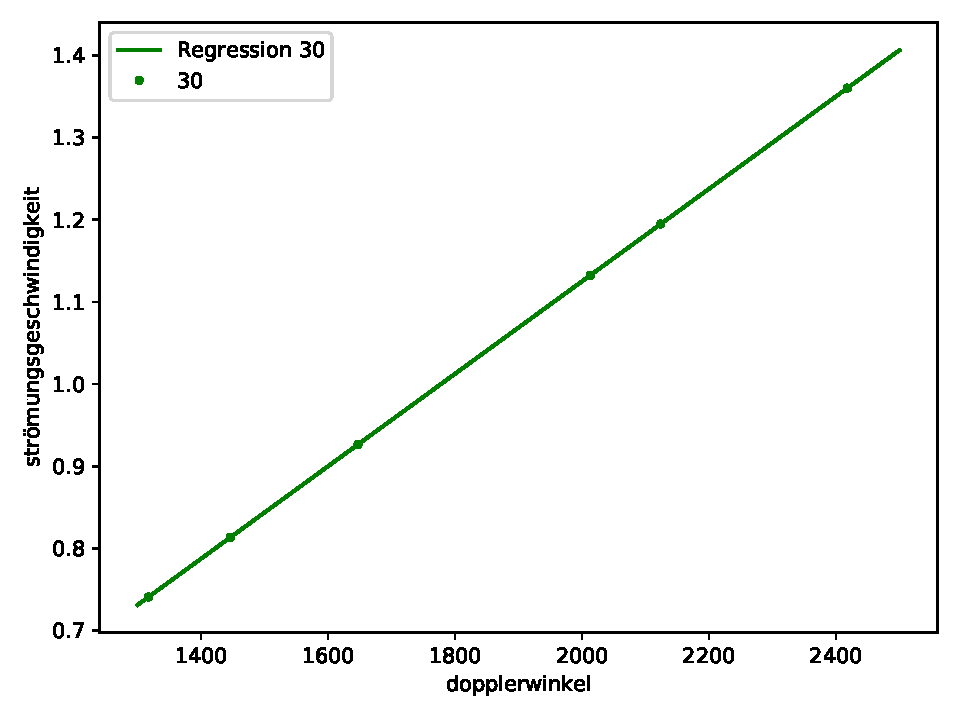
\includegraphics[width=\textwidth]{build/plot2.pdf}
    \caption{Temperaturdifferenz $T_{St}$ zwischen dem breiten Messingstab und dem Edelstahlstab.}
    \label{fig:diff}
\end{figure}

\noindent
Es ist zu erkennen, dass die Temperaturdifferenz für beide Metalle zu Beginn nahe null ist. Beide Graphen steigen dann stark an, bis sie
nach einem Maximum abflachen und sich einer konstanten Grenztemperatur nähern. Die Kurve des Messingstabes erreicht dabei das Maximum früher
und der Funktionswert ist deutlich geringer als bei der Edelstahlkurve. Auch die Grenztemperatur des Edelstahl ist deutlich größer als die des
Messings.

\subsection{Dynamische Methode}
\label{sec:ad}
In Abbildung \ref{fig:messing} sind die Temperaturverläufe des breiteren Messingstabes graphisch aufgetragen. Dabei wurde der Stab nach Kapitel
\ref{sec:dynamisch} mit einer Periodendauer von $\SI{80}{\second}$ geheizt.

\begin{figure}[H]
    \centering
    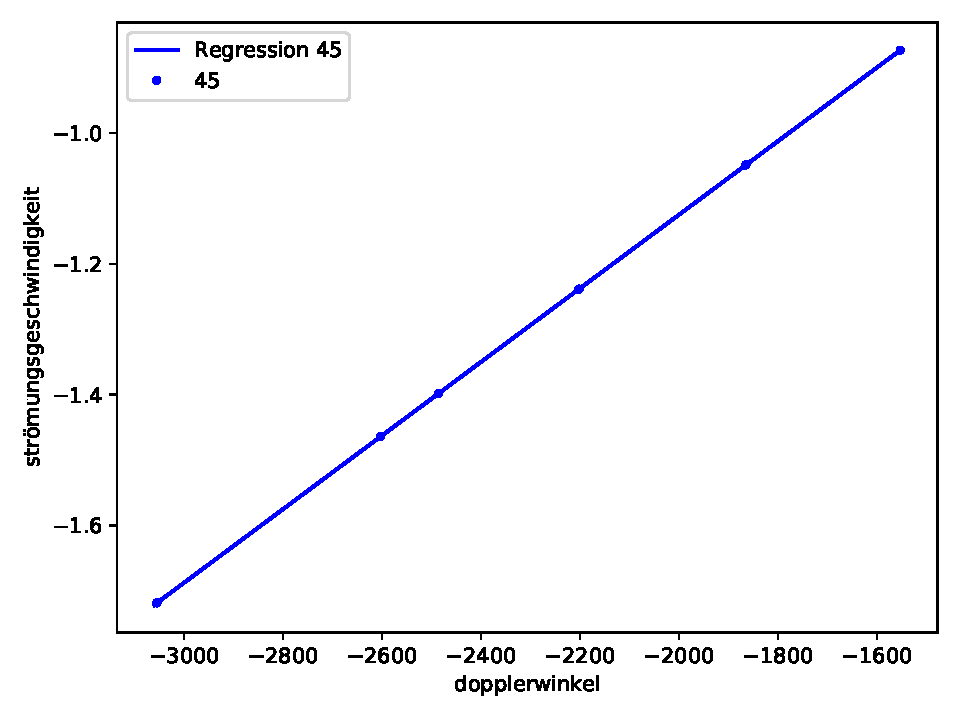
\includegraphics[width=\textwidth]{build/plot3.pdf}
    \caption{Temperaturverläufe des breiteren Messingstabes mit einer Periodendauer von $\SI{80}{\second}$.}
    \label{fig:messing}
\end{figure}
\noindent
Aus dem Graphen werden mittels \textit{scipy.signal} \cite{scipy} die Amplituden $A_\text{nah}$ und $A_\text{fern}$ und die Phasenverschiebung $\Delta t$ zwischen
$T_\text{nah}$ und $T_\text{fern}$ bestimmt. Diese Werte sind in Tabelle \ref{tab:messing}  aufgelistet.

\begin{table}[H]
    \centering
        \caption{Amplituden $A$ und Phasenverschiebung $\Delta t$ von Messing.}
        \label{tab:messing}
        \sisetup{table-format=1.2}
        \begin{tabular}{S S[table-format=1.2] S[table-format=2.1] S[table-format=2.2]}
          \toprule
          {$A_\text{nah}[\si{\kelvin}]$} & {$A_\text{fern}[\si{\kelvin}]$} & {$\Delta t[\si{\second}]$} & {$\kappa [\si{\watt\per\milli\kelvin}]$}\\
          \midrule
          5.99&      0.10&     28.5&     12.39\\
          6.92&      0.57&     20.5&     28.24\\
          7.27&      0.92&     19.0&     36.80\\
          7.57&      1.18&     16.0&     48.60\\
          7.83&      1.39&     15.0&     55.74\\
          8.00&      1.57&     14.5&     61.22\\
          8.06&      1.68&     14.5&     63.57\\
          7.55&      1.92&     18.5&     57.06\\
          8.34&      1.84&     13.5&     70.85\\
          8.31&      1.92&     13.5&     73.08\\
          \bottomrule
        \end{tabular}
      \end{table}

\noindent
Vollkommen analog sind in Abbildung \ref{fig:alu} die Temperaturverläufe für Aluminium dargestellt. Die abgelesenen Werte finden sich in
Tabelle \ref{tab:alu}.

\begin{figure}[H]
    \centering
    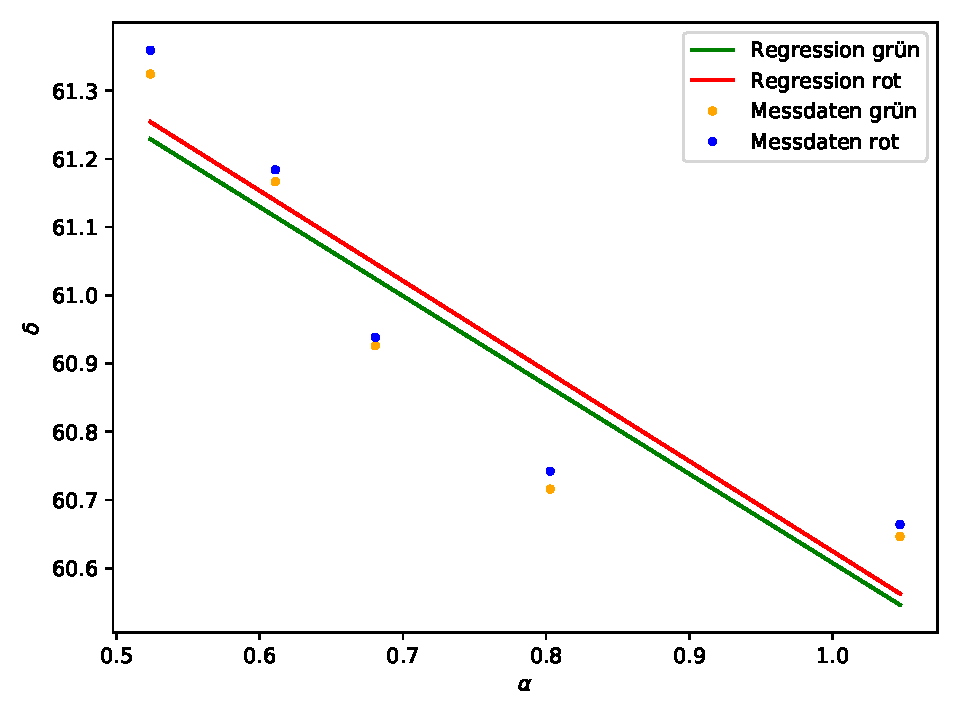
\includegraphics[width=\textwidth]{build/plot4.pdf}
    \caption{Temperaturverläufe des Aluminiumstabes mit einer Periodendauer von $\SI{80}{\second}$.}
    \label{fig:alu}
\end{figure}
\noindent

\begin{table}[H]
    \centering
        \caption{Amplituden $A$ und Phasenverschiebung $\Delta t$ von Aluminium.}
        \label{tab:alu}
        \sisetup{table-format=2.2}
        \begin{tabular}{S S S[table-format=2.0] S[table-format=3.2]}
          \toprule
          {$A_\text{nah}[\si{\kelvin}]$} & {$A_\text{fern}[\si{\kelvin}]$} & {$\Delta t[\si{\second}]$} & {$\kappa [\si{\watt\per\milli\kelvin}]$}\\
          \midrule
           9.06&      2.26&     11.5&     70.78\\
          10.73&      3.96&      8.5&    133.39\\
          11.20&      4.53&      7.5&    166.48\\
          11.47&      4.85&      7.0&    187.58\\
          11.68&      5.03&      7.0&    191.65\\
          11.79&      5.29&      7.0&    201.46\\
          11.79&      5.20&      7.0&    197.24\\
          11.25&      5.18&     14.0&    104.09\\
          11.97&      5.31&      7.0&    198.64\\
          11.94&      5.36&      7.0&    201.59\\
          \bottomrule
        \end{tabular}
      \end{table}
\noindent
Mit
\begin{equation}
  \bar{x}=\frac{1}{n}\sum_{i=1}^n{x_i}
  \label{eqn:Mittelwert}
\end{equation}
und
\begin{align}
  \sigma&=\sqrt\frac{1}{(N-1)}\sum_{k=1}^N\!(x_k-\bar{x})^2 \label{eqn:Standardabweichung}\\
  \Delta\bar{x}&=\frac{\sigma}{\sqrt{n}} \label{eqn:Standardfehler}
\end{align}
lassen sich nun die Mittelwerte und die zugehörigen Unsicherheiten berechnen. Es ergibt sich für den breiten Messingstab
\begin{align*}
  \bar{A}_\text{messing,b,fern} &=\SI{1.31 \pm 0.62}{\kelvin}\\
  \bar{A}_\text{messing,b,nah}  &=\SI{7.58 \pm 0.72}{\kelvin}\\
  \olsi{\Delta t}_\text{messig} &=\SI{17.35\pm 4.61}{\second}\\
\end{align*}
und für den Aluminiumstabe
\begin{align*}
  \bar{A}_\text{alu,fern}       &=\SI{4.70 \pm 0.96}{\kelvin}\\
  \bar{A}_\text{alu,nah}        &=\SI{11.29\pm 0.87}{\kelvin}\\
  \olsi{\Delta t}_\text{alu}    &=\SI{8.36 \pm 2.44}{\second}\;.
\end{align*}
Mit Gleichung \eqref{eqn:wärmeleitfähigkeit} kann nun die Wärmeleitfähigkeit $\kappa$ bestimmt werden. Die zugehörige Unsicherheit wird mit der Gauß'schen
Fehlerfortpflanzung
\begin{equation}
  \Delta f = \sqrt{\sum_{i=1}^N
  \left(\frac{\partial f}{\partial x_i}\right)^2
  (\Delta x_i)^2}.
  \label{eqn:GaußFehler}
\end{equation}
mit den Unsicherheiten $\Delta A$ und $\Delta t$. Es folgt
\begin{equation*}
  \Delta\kappa=\sqrt{
    \left(  \frac{\rho c (\Delta x)^2}{2\Delta t \ln{\left(\frac{\bar{A}_\text{nah}}{\bar{A}_\text{fern}}\right)^2}} \right)^2
    \left(  \left(\frac{\Delta\bar{A}_\text{fern}}{\bar{A}_\text{fern}} \right)
    +\left( \frac{\Delta\bar{A}_\text{fern}}{\bar{A}_\text{fern}}  \right) \right)
    +\left( \frac{\rho c (\Delta x)^2}{(\olsi{\Delta t})^2\ln{\left(\frac{\bar{A}_\text{nah}}{\bar{A}_\text{fern}}\right)}}\right)
    \left(  \Delta\olsi{\Delta t}\right)^2
  }\;.
\end{equation*}
Damit ergeben sich für die Wärmeleitfähigkeiten von Messing und Aluminium
\begin{align*}
  \kappa_\text{messing}&=\SI{47.42\pm 12.61}{\watt\per\metre\per\kelvin}\\
  \kappa_\text{alu}    &=\SI{154.4\pm 45.1}{\watt\per\metre\per\kelvin}  \;.
\end{align*}

\noindent
Für Edelstahl ist das Vorgehen recht analog, nur die Periodendauer ist nach Kapitel \ref{sec:dynamisch} auf $\SI{200}{\second}$ erhöht.
In Abbildung \ref{fig:stahl} sind die Temperaturverläufe der Thermoelemente dargestellt.

\begin{figure}[H]
    \centering
    \includegraphics[width=\textwidth]{build/plot5.pdf}
    \caption{Temperaturverläufe des Edelstahlstabes mit einer Periodendauer von $\SI{200}{\second}$.}
    \label{fig:stahl}
\end{figure}
\noindent
Die Amplituden und Phasendifferenzen werden abermals mit \textit{scipy.signal} \cite{scipy} ausgewertet und sind in Tabelle \ref{tab:stahl}
dargestellt.

\begin{table}[H]
    \centering
        \caption{Amplituden $A$ und Phasenverschiebung $\Delta t$ von Edelstahl.}
        \label{tab:stahl}
        \sisetup{table-format=2.2}
        \begin{tabular}{S S S[table-format=2.0] S}
          \toprule
          {$A_\text{nah}[\si{\kelvin}]$} & {$A_\text{fern}[\si{\kelvin}]$} & {$\Delta t[\si{\second}]$} & {$\kappa [\si{\watt\per\milli\kelvin}]$}\\
          \midrule
          15.75&      0.10&     81&      3.51\\
          16.53&      0.42&     71&      5.52\\
          17.07&      0.72&     63&      7.22\\
          17.47&      1.00&     58&      8.68\\
          17.82&      1.30&     55&     10.00\\
          18.02&      1.52&     52&     11.09\\
          18.18&      1.71&     50&     12.18\\
          18.46&      1.86&     49&     12.80\\
          \bottomrule
        \end{tabular}
      \end{table}
\noindent
Die Mittelwerte und deren Unsicherheiten sind nach den Gleichungen \eqref{eqn:Mittelwert} und %\eqref{eqn:Standardehler}
\begin{align*}
  \bar{A}_\text{stahl}         &=\SI{17.41 \pm 0.92}{\kelvin}\\
  \bar{A}_\text{stahl}         &=\SI{1.08  \pm 0.63}{\kelvin}\\
  \olsi{\Delta t}_\text{stahl} &=\SI{59.94\pm 11.19}{\second} \;.
\end{align*}
Die Wärmeleitfähigkeit ist dann nach Gleichung \eqref{eqn:wärmeleitfähigkeit} und \eqref{eqn:GaußFehler}
\begin{equation*}
  \kappa_\text{stahl}=\SI{8.64 \pm 1.61}{\watt\per\metre\per\kelvin}  \;.
\end{equation*}
Die Wellenlänge der Temperaturwelle wird mit Gleichung \eqref{eqn:phasengeschwindigkeit} berechnet, wobei
\begin{equation*}
  \omega=\frac{2\pi}{T}
\end{equation*}
mit den Periodendauern $T_1=\SI{80}{\second}$ und $T_2=\SI{200}{\second}$ ausgenutzt wird, sodass die Wellenlänge durch
\begin{equation*}
  \lambda=\sqrt{\frac{4\pi\kappa T}{\rho c}}
\end{equation*}
ausgedrückt wird. Einsetzen ergibt
\begin{align*}
\lambda_\text{messing} &=\SI{0.122\pm 0.016}{\metre}\\
\lambda_\text{alu}     &=\SI{0.249\pm 0.036}{\metre}\\
\lambda_\text{stahl}   &=\SI{0.052\pm 0.005}{\metre}   \;.
\end{align*}
